\setlength{\tabcolsep}{8pt}
\begin{table*}[t]

\newcommand{\first}{\cellcolor{red!40}}
\newcommand{\second}{\cellcolor{orange!40}}
\newcommand{\third}{\cellcolor{yellow!40}}
\setlength{\tabcolsep}{4pt}

\centering
\resizebox{\textwidth}{!}{

\begin{tabular}{l|rrrrr|rrrrr}
\toprule
\multicolumn{1}{c|}{} & \multicolumn{5}{|c|}{MipNeRF 360 (3 scenes)} & \multicolumn{5}{|c}{LLFF (7 scenes)} \\
\midrule
Method       & PSNR $\uparrow$ & SSIM $\uparrow$ & LPIPS $\downarrow$ & Time (min.) $\downarrow$ & ATE     & PSNR $\uparrow$ & SSIM $\uparrow$ & LPIPS $\downarrow$ & Time (min.) $\downarrow$ & ATE     \\
\midrule
FlowMap      &   \third{29.84} &   \third{0.916} &      \third{0.073} &             \third{19.8} & 0.00055 &  \second{27.23} &   \third{0.849} &     \second{0.079} &              \third{7.5} & 0.00209 \\
COLMAP       &  \second{29.95} &  \second{0.928} &              0.074 &             \second{4.8} &     N/A &           25.73 &  \second{0.851} &              0.098 &             \second{1.1} &     N/A \\
COLMAP (MVS) &   \first{31.03} &   \first{0.938} &      \first{0.060} &                     42.5 &     N/A &   \first{27.99} &   \first{0.867} &      \first{0.072} &                     13.4 &     N/A \\
DROID-SLAM*  &           29.83 &           0.913 &     \second{0.066} &              \first{0.6} & 0.00017 &   \third{26.21} &           0.818 &      \third{0.094} &              \first{0.3} & 0.00074 \\
NoPE-NeRF*   &           13.60 &           0.377 &              0.750 &                   1913.1 & 0.04429 &           17.35 &           0.490 &              0.591 &                   1804.0 & 0.03920 \\
\midrule
\multicolumn{1}{c|}{} & \multicolumn{5}{|c|}{Tanks \& Temples (14 scenes)} & \multicolumn{5}{|c}{CO3D (2 scenes)} \\
\midrule
Method       & PSNR $\uparrow$ & SSIM $\uparrow$ & LPIPS $\downarrow$ & Time (min.) $\downarrow$ & ATE     & PSNR $\uparrow$ & SSIM $\uparrow$ & LPIPS $\downarrow$ & Time (min.) $\downarrow$ & ATE     \\
\midrule
FlowMap      &  \second{27.00} &  \second{0.854} &     \second{0.101} &             \third{22.3} & 0.00124 &   \first{31.11} &   \first{0.896} &      \first{0.064} &             \third{22.1} & 0.01589 \\
COLMAP       &   \third{26.74} &   \third{0.848} &      \third{0.130} &             \second{5.5} &     N/A &           25.17 &           0.750 &              0.190 &            \second{12.6} &     N/A \\
COLMAP (MVS) &   \first{27.43} &   \first{0.863} &      \first{0.097} &                     51.4 &     N/A &   \third{25.35} &   \third{0.762} &      \third{0.175} &                     52.0 &     N/A \\
DROID-SLAM*  &           25.70 &           0.824 &              0.133 &              \first{0.8} & 0.00122 &  \second{25.97} &  \second{0.790} &     \second{0.139} &              \first{0.8} & 0.01728 \\
NoPE-NeRF*   &           13.38 &           0.449 &              0.706 &                   2432.9 & 0.03709 &           14.97 &           0.400 &              0.770 &                   2604.9 & 0.03648 \\
\bottomrule
\end{tabular}
}

\vspace{5pt}
\caption{Camera parameter and geometry intializations from FlowMap produce 3D Gaussian reconstruction results that far outperform prior gradient-based baselines and are generally on par with those produced by COLMAP. Methods marked with an asterisk require ground-truth intrinsics. We report ATE with respect to COLMAP's pose estimates for reference, since no ground-truth trajectories exist for common view synthesis datasets. We exclude scenes where COLMAP or FlowMap fail entirely; each fails on 4 scenes. See the supplementary document for more details.}
\label{tab:recon}
\vspace{-11pt}
\end{table*}

\begin{figure*}[t]
    \centering
    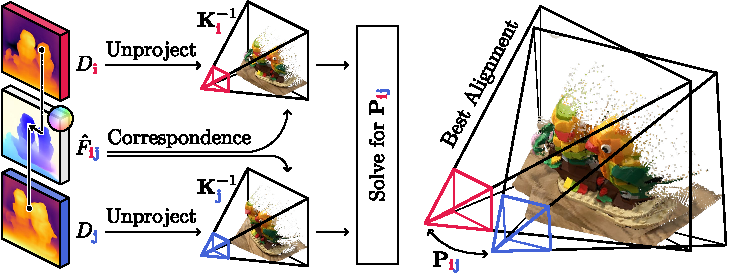
\includegraphics[width=\linewidth,]{figures/procrustes/fig_procrustes_pdf_small.pdf}
    \vspace{-12pt}
    \caption{We solve for the relative poses between consecutive frames using their depth maps, camera intrinsics, and optical flow. To do so, we first unproject their depth maps, then solve for the pose that best aligns the resulting point clouds.}
    \label{fig:procrustes}
    \vspace{-15pt}
\end{figure*}

\begin{figure*}[t]
    \centering
    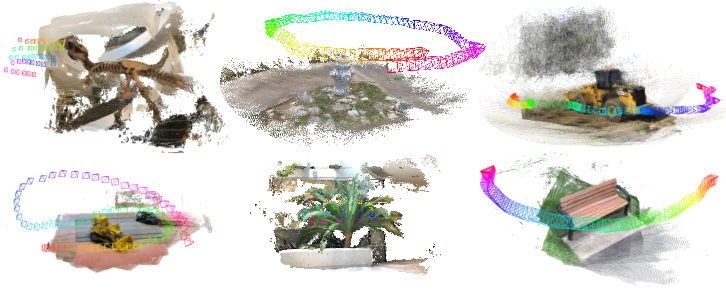
\includegraphics[width=\linewidth]{figures/pdfs/point_clouds_small.pdf}
    \caption{\textbf{Point Clouds Reconstructed by FlowMap.} Unprojecting FlowMap depths using FlowMap's intrinsics and poses yields dense and consistent point clouds.}
    \label{fig:point_clouds}
    \vspace{-10pt}
\end{figure*}


\section{Results}
\label{sec:exp}

We benchmark FlowMap via the downstream task of 3D Gaussian reconstruction~\cite{kerbl20233d}.
This allows us to measure the quality of the camera parameters and geometry (depth maps) it outputs \emph{without having access to ground-truth scene geometry and camera parameters}.


\myparagraph{Baselines.}
We benchmark FlowMap against several baselines.
First, we evaluate against COLMAP~\cite{schonberger2016structure}, the state-of-the-art structure-from-motion (SfM) method.
Given a collection of images, COLMAP outputs per-image camera poses and intrinsics alongside a sparse 3D point cloud of the underlying scene.
3D Gaussian Splatting, which was designed around COLMAP's SfM outputs, is initialized using this point cloud.
Second, we evaluate against COLMAP multi-view stereo (MVS), which enhances COLMAP's output with a much denser 3D point cloud.
When initialized using this denser point cloud, 3D Gaussian Splatting produces slightly better results.
However, note that COLMAP MVS is rarely used in practice because it can be prohibitively time-consuming to run.
Third, we evaluate against DROID-SLAM, a neural SLAM system trained on a synthetic dataset of posed video trajectories.
Finally, we evaluate against NoPE-NeRF, an method that jointly optimizes a neural radiance field and unknown camera poses.
Note that unlike FlowMap and COLMAP, both DROID-SLAM and NoPE-NeRF require camera intrinsics as input.

\myparagraph{Datasets.}

We analyze FlowMap on four standard novel view synthesis datasets: MipNeRF-360~\cite{barron2021mipnerf}, Tanks \& Temples~\cite{Knapitsch2017tanks}, LLFF~\cite{mildenhall2019local}, and CO3D~\cite{reizenstein2021common}.
Because FlowMap runs on video sequences, we restrict these datasets to just the video-like sequences they provide.

\myparagraph{Methodology.}

We run FlowMap and the baselines using images that have been rescaled to a resolution of about 700,000 pixels.
We then optimize 3D Gaussian scenes for all methods except NoPE-NeRF, since it provides its own NeRF renderings.
We use 90\% of the available views for training and 10\% for testing.
During 3D Gaussian fitting, we follow the common~\cite{nerfstudio} practice of fine-tuning the initial camera poses and intrinsics.
Such refinement is beneficial because the camera poses produced by SfM algorithms like COLMAP are generally not pixel-perfect~\cite{park2023camp,lin2021barf}.
We use the 3D points provided by COLMAP, DROID-SLAM, and FlowMap as input to 3D Gaussian Splatting.
For FlowMap, we combine the output depth maps, poses, and intrinsics to yield one point per depth map pixel.

\subsection{Novel View Synthesis Results}

Tab.~\ref{tab:recon} reports rendering quality metrics (PSNR, SSIM, and LPIPS) on the held-out test views, and Fig.~\ref{fig:splat_comparison} shows qualitative results.
Qualitatively, FlowMap facilitates high-quality 3D reconstructions with sharp details.
Quantitatively, FlowMap performs slightly better than COLMAP SfM and significantly outperforms DROID-SLAM and NoPE-NeRF.
Only COLMAP MVS slightly exceeds FlowMap in terms of reconstruction quality.
As noted previously, COLMAP MVS is rarely used for 3D Gaussian Splatting, since it is very time-consuming to run on high-resolution images.

\subsection{Camera Parameter Estimation Results}

Since the datasets we use do not provide ground-truth camera parameters, they cannot be used to directly evaluate camera parameter estimates.
Instead, Tab.~\ref{tab:recon} reports the average trajectory error (ATE) of FlowMap, DROID-SLAM, and NoPe-NeRF with respect to COLMAP.
Since COLMAP's poses are not perfect~\cite{park2023camp}, this comparison is not to be understood as a benchmark, but rather as an indication of how close these methods' outputs are to COLMAP's state-of-the-art estimates.
We find that DROID-SLAM and FlowMap both recover poses that are close to COLMAP's, while NoPE-NeRF's estimated poses are far off.
When computing ATEs, we normalize all trajectories such that $\text{tr}(XX^T) = 1$, where $X$ is an $n$-by-3 matrix of camera positions.

Fig.~\ref{fig:trajectories} plots trajectories recovered by FlowMap against those recovered by COLMAP, showing that they are often nearly identical.
Fig.~\ref{fig:point_clouds} shows point clouds derived from FlowMap's estimated depth maps and camera parameters, illustrating that FlowMap recovers well-aligned scene geometry.

\subsection{Large-Scale Robustness Study}

\begin{figure*}[t!]
    \centering
    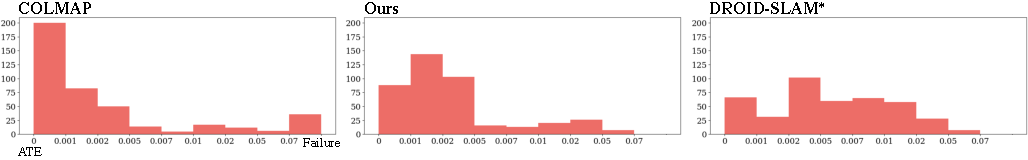
\includegraphics[width=\linewidth,]{figures/pdfs/colmap_study_hist.pdf}
    \vspace{-20pt}
    \caption{\textbf{Large-scale Robustness Study.}
    We run FlowMap and DROID-SLAM on 420 CO3D scenes across 10 categories and plot mean ATEs with respect to CO3D's COLMAP-generated pose metadata.
    We also re-run COLMAP on the same data.
    Compared to DROID-SLAM, which requires ground-truth intrinsics, FlowMap produces notably lower ATEs.
    FlowMap's ATE distribution is similar to one obtained by re-running COLMAP, with most ATEs falling under 0.005 in both cases.}
    \label{fig:colmap_study}
    \vspace{-5pt}
\end{figure*}


We study FlowMap's robustness by using it to estimate camera poses for 420 CO3D scenes from 10 categories.
We compare these trajectories to CO3D's pose annotations, which were computed using COLMAP.
Since the quality of CO3D's ground-truth trajectories varies between categories, we focus on categories that have been used to train novel view synthesis models~\cite{tewari2023diffusion,chan2023generative,wewer24latentsplat}, where pose accuracy is expected to be higher.
We find that FlowMap's mean ATE (0.0056) is lower than DROID-SLAM's (0.0082) and similar to the mean ATE obtained by re-running COLMAP and comparing the results to the provided poses (0.0038).
This demonstrates that FlowMap consistently estimates poses which are close to COLMAP's.
We note that COLMAP failed to estimate poses for 36 scenes, possibly because we ran it at a sparser frame rate to be consistent with our method or because the original annotations were generated using different COLMAP settings; we exclude COLMAP's failures from the above mean ATE.
See Fig.~\ref{fig:colmap_study} for distributions of ATE values with respect to CO3D's provided camera poses.
\vspace{-10pt}
